This report presents a length-based assessment of the multi-species deep slope fisheries targeting mostly snappers, groupers and emperors, at depths ranging from 50 to 500 meters, in fisheries management areas (WPP) 714 and 715 in eastern Indonesia. These WPPs cover the Maluku, Seram, Banda and Flores Seas and they were combined as a single area for analysis, as the border between WPP 714 and WPP 715 cuts through the middle of the fishing grounds. Drop line and mini long line vessels fish on both sides of this border sometimes even within a single fishing trip. Also in terms of habitat and ecology of the target species the 2 WPPs covered in this report are very similar and completely connected. Fishing grounds for snappers, groupers, emperors and other target species in this region include deep slopes along the many islands as well as seamounts and other deep structures which are characteristic for this area.

Several fleets from this region contributed data to the current assessment, including a medium scale drop line fishery based in Kema (20 boats), North Sulawesi, and a small scale mini long line fishery based in the Banggai and Sula Islands on the border of the Maluku and Banda Seas. In addition, data were used from fleets originating from outside the region (e.g. Bali, Probolinggo, Kupang) but operating inside WPP 714 and/or WPP715. Fishing grounds for the small scale mini long line fleet are concentrated near the home islands near the center of our area of interest, whereas the medium scale drop liners from Kema make trips to locations up to 1,000 kilometers away from their port, to all corners of this region.

Kema based vessels make up to about 10 trips a year, landing around 4 tons of mixed snapper, grouper and emperor for each trip or up to about 40 tons per vessel per year. The drop line fishery is an active vertical hook and line fishery operating at depths from 50 to 500 meters, whereas long lines are set horizontally along the bottom at depths ranging from 50 to 150 meters. This report analyzes length frequencies of the 50 species of fish that were the most abundant in the combined drop and long line fisheries operating in WPP 714 and WPP 715. For a complete overview of the species composition please refer to the ID guide prepared for these fisheries:

\textbf{CLICK: }\href{http://72.14.187.103:8080/ifish/pub/TNC_FishID.pdf}{Link to on-line E-Book Species ID Guide}

For further background on species life history characteristics, and data-poor length based assessment methods, as applied in this report, please refer to the assessment guide that was separately prepared for these fisheries:

\textbf{CLICK: }\href{http://72.14.187.103:8080/ifish/pub/DeepSlopeSpeciesAssessmentTool.pdf}{Link to on-line E-Book Assessment Guide with Biological Information}

Data in this report represent complete catches by small and medium scale vessels from the above described fleets. All fish captured were photographed on measuring boards by fishing crew participating in our Crew Operated Data Recording System or CODRS. Images were analyzed by project staff to generate the species specific length frequency distributions of the catches which served as the input for our length based assessment of this fishery.

\begin{center}
\graphicspath{{/root/R-project/IFishSnapperWPP714_715/Images/}}
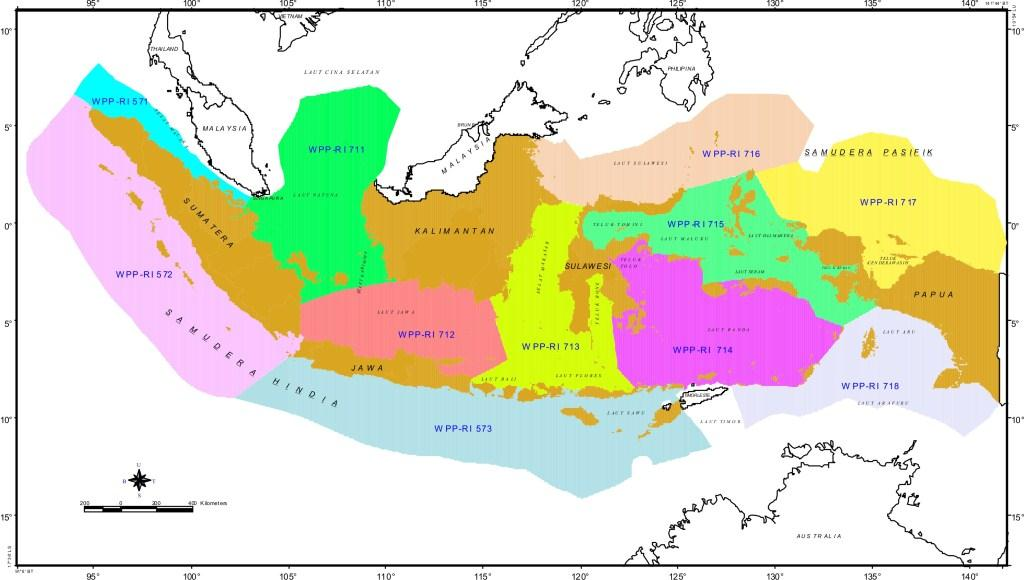
\includegraphics[scale=1.8]{wpp-indonesia.jpg}

Figure 1. Fisheries Management Areas (WPP) in Indonesian marine waters.
\end{center}

\begin{center}
\graphicspath{{/root/R-project/IFishSnapperWPP714_715/Images/}}
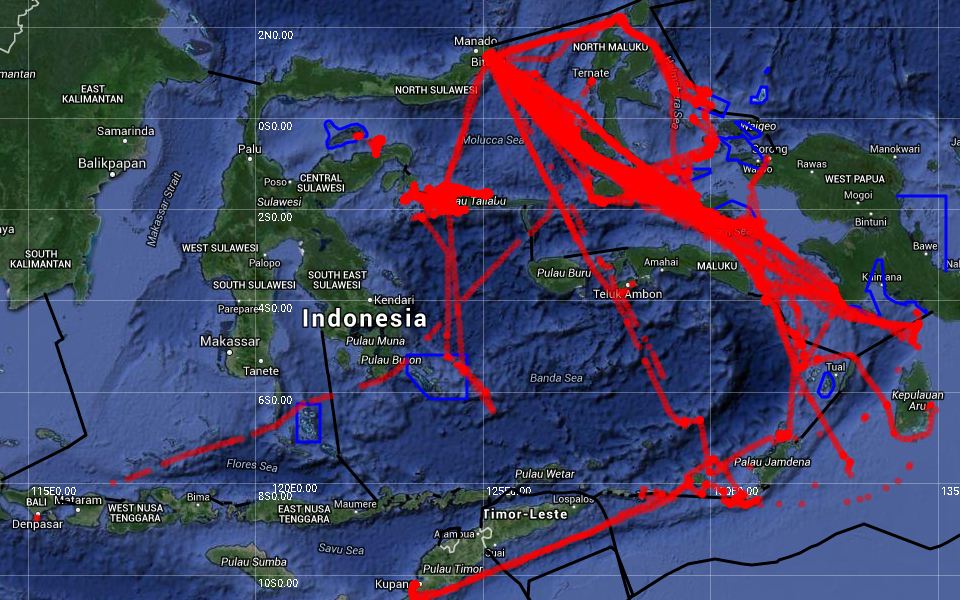
\includegraphics[scale=0.6]{SpotTrace-AreaC-Satellite.jpg}

Figure 2. Map with fishing ground bathymetry and tracks (in red) of snapper fishing trips into WPP 714 and 715. Black lines are WPP boundaries, blue lines are MPA boundaries. This figure mainly represents fleets from Kema (near Manado) and the Banggai / Sula Islands.
\end{center}